\documentclass{boi2014-pl}

\usepackage{enumitem}
\usepackage{todonotes}
\usepackage{wrapfig}
\usepackage{mathtools}
\usepackage{tikz}

\renewcommand{\DayNum}{1}
\renewcommand{\TaskCode}{coprobber}
\renewcommand{\TaskName}{Policjant i złodziej}
\renewcommand{\TaskVersion}{1.3}

\renewcommand{\labelitemii}{$\circ$}
\newcommand{\param}[1]{{\tt #1}}
\renewcommand{\method}[1]{{\tt #1}}
\newcommand{\constant}[1]{{\tt #1}}

\begin{document}
    \begin{wrapfigure}[8]{r}{6cm}
        \vspace{-24pt}
		\includegraphics[width=6cm]{\TaskCode.jpeg}
	\end{wrapfigure}

  \medskip
    Przestępczość w Bajtogrodzie jest na porządku dziennym.
    Szczególnie często mają miejsce kradzieże.
    Jedną z przyczyn tego stanu rzeczy może być fakt, iż w pogoń za złodziejem
    rusza zazwyczaj tylko jeden policjant znajdujący się akurat w terenie.
    Pościg w staroświeckim stylu odbywa się wąskimi uliczkami łączącymi
    \emph{skrzyżowania} Bajtogrodu, a dzięki dobrej znajomości miasta złodziejowi
    nierzadko udaje się umknąć policjantowi.

  \smallskip
    Komenda Stołeczna Policji w Bajtogrodzie (KSPB) organizuje zgrupowanie poświęcone
    zmniejszeniu skali przestępczości w mieście.
    Jednym z pomysłów jest wprowadzenie automatycznego systemu planowania tras pościgu
    za złodziejami.
    W tym celu KSPB zdobyło już dokładny plan miasta.
    Teraz poproszono Cię, abyś przygotował program, który korzystając z tych danych,
    umożliwi efektywne planowanie pościgu.

    Pościg policjanta za złodziejem modelujemy następująco:
    \begin{enumerate}
        \item Policjant wybiera skrzyżowanie, na którym rozpoczyna swój patrol.
        \item Następnie złodziej wybiera skrzyżowanie, przy którym dokona włamania
            (wie on, na którym skrzyżowaniu znajduje się policjant).
            Od tego momentu zakładamy, że policjant i złodziej znają wzajemnie
            swoje położenia.
        \item W pojedynczym ruchu policjant przemieszcza się na sąsiednie skrzyżowanie
            (tzn.\ skrzyżowanie połączone bezpośrednio uliczką ze skrzyżowaniem,
            na którym jest obecnie) lub decyduje się czekać (tzn.\ nie przemieszcza się).
        \item W pojedynczym ruchu złodziej przemieszcza się na sąsiednie skrzyżowanie.
            Zauważ, że w przeciwieństwie do policjanta, złodziej nigdy nie czeka
            w swoim ruchu.
            Na złodzieju czapka gore.
        \item Policjant i złodziej wykonują ruchy na przemian (począwszy od policjanta),
            aż do momentu, gdy:
        \begin{enumerate}
            \item wcześniejsza sytuacja powtórzy się (przez sytuację rozumiemy pozycje
                obu graczy oraz to, do którego gracza należy najbliższy ruch).
                Oznacza to, że złodziej może unikać spotkania z policjantem w nieskończoność,
                więc przyjmujemy, że złodziej uciekł policjantowi; albo
            \item policjant i złodziej spotkają się na tym samym skrzyżowaniu
                po ruchu któregoś z nich.
                Wówczas policjant łapie złodzieja.
        \end{enumerate}
    \end{enumerate}

    \Task
    Napisz program, który mając dany plan miasta, stwierdzi, czy policjant może
    złapać złodzieja, a jeśli tak, przeprowadzi pościg w imieniu policjanta.

    Twój program powinien założyć, że złodziej porusza się w sposób optymalny.

    \Implementation
    Powinieneś zaimplementować dwie funkcje:
    \begin{itemize}
        \item \method{start(N, A)} o następujących parametrach:
            \begin{itemize}
                \item $N$ -- liczba skrzyżowań (skrzyżowania są ponumerowane od $0$ do $N-1$)
                \item $A$ -- dwuwymiarowa tablica opisująca uliczki;
                    dla $0 \le i, j \le N-1$,
                    $$
                        A[i, j] \text{ jest równe }
                        \begin{dcases*}
                            \texttt{false} & jeśli skrzyżowania $i$ oraz $j$ nie są połączone uliczką
                                \\
                            \texttt{true} & jeśli skrzyżowania $i$ oraz $j$ są połączone uliczką.
                        \end{dcases*}
                    $$
                    Wszystkie uliczki są dwukierunkowe (tzn.\ $A[i, j] = A[j, i]$
                    dla wszystkich $i$ oraz $j$) i każda uliczka łączy dwa różne skrzyżowania
                    (tzn.\ $A[i, i]$ będzie równe \texttt{false} dla wszystkich $i$).
                    Możesz ponadto założyć, że za pomocą systemu uliczek można przedostać
                    się z dowolnego skrzyżowania na dowolne inne skrzyżowanie.
            \end{itemize}

        Jeśli w tak opisanym mieście policjant może złapać złodzieja,
        wynikiem funkcji \method{start} powinien być numer skrzyżowania,
        na którym policjant powinien rozpocząć swój patrol.
        W przeciwnym razie wynikiem funkcji powinno być $-1$.

        \item \method{nextMove(R)} przyjmującą jako parametr liczbę
            $R$ oznaczającą numer skrzyżowania, przy którym znajduje się złodziej,
            i zwracającą numer skrzyżowania, przy którym policjant znajdzie się
            po wykonaniu swojego ruchu.
    \end{itemize}

    Funkcja \method{start} zostanie wywołana dokładnie raz,
    przed wszystkimi wywołaniami funkcji \method{nextMove}.
    Jeśli wynikiem funkcji \method{start} będzie $-1$,
    funkcja \method{nextMove} nie będzie wywoływana.
    W przeciwnym razie, funkcja \method{nextMove} będzie wywoływana w kółko
    aż do końca pościgu.
    Program zakończy się, gdy spełniony zostanie jeden z poniższych warunków:
    \begin{itemize}
        \item funkcja \method{nextMove} zwróci niepoprawny ruch;
        \item wcześniejsza sytuacja powtórzy się;
        \item złodziej zostanie złapany.
    \end{itemize}

    \Example
    \begin{wrapfigure}[4]{r}{2cm}
        \vspace{-0.5cm}
        \centering
        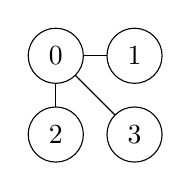
\begin{tikzpicture}
        \draw (0,1) -- (0,0);
        \draw (0,1) -- (1,0);
        \draw (0,1) -- (1,1);
        \foreach \x in {0,1} \foreach \y in {0,1}
            \draw (\x,\y) node[circle,draw,fill=white,inner sep=0,minimum size=0.7cm] {\pgfmathparse{int(2-2*\y+\x)}\pgfmathresult};
        \end{tikzpicture}
    \end{wrapfigure}
    Przyjrzyjmy się przykładowi opisanemu przez obrazek po prawej.
    W tym przykładzie każde skrzyżowanie jest dobrą pozycją początkową dla policjanta.
    Jeśli policjant rozpocznie patrol przy skrzyżowaniu numer 0, w swoim pierwszym ruchu
    może czekać -- wówczas złodziej sam na niego wpadnie.
    Jeśli zaś policjant rozpocznie patrol przy jakimkolwiek innym skrzyżowaniu, może poczekać,
    aż złodziej znajdzie się przy skrzyżowaniu numer 0, i wówczas przejść na to skrzyżowanie.
   
    Oto jedno z możliwych wykonań programu dla tego przykładu:

    \begin{tabular}{|l|c|}
        \hline
            {\bf Wywołanie funkcji} & {\bf Wynik} \\
        \hline
            \method{start(4, [[0, 1, 1, 1], [1, 0, 0, 0], [1, 0, 0, 0], [1, 0, 0, 0]])} &
            \constant{3} \\
        \hline
            \method{nextMove(1)} & \constant{3} \\
        \hline
            \method{nextMove(0)} & \constant{0} \\
        \hline
    \end{tabular}

    Uwaga: w powyższym wywołaniu funkcji \method{start} liczba \constant{0} oznacza
    \constant{false} a liczba \constant{1} oznacza \constant{true}.

    \Scoring
    \begin{description}
        \item[Podzadanie 1 (16 punktów):] $2 \le N \le 500$. Każda para skrzyżowań jest połączona za pomocą dokładnie jednej ścieżki złożonej z uliczek.
        \item[Podzadanie 2 (14 punktów):] $2 \le N \le 500$. Sieć skrzyżowań i uliczek tworzy kratkę.
        Kratka składa się z co najmniej dwóch wierszy i kolumn, a numeracja skrzyżowań
        odpowiada schematowi przedstawionemu na rysunku poniżej.
        \begin{figure}[h!]
           \centering
           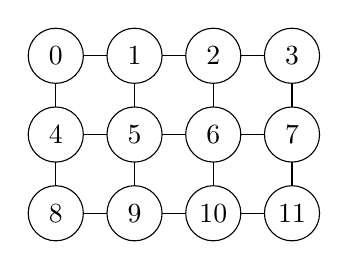
\begin{tikzpicture}
            \draw (0,0) grid (3,2);
            \foreach \x in {0,1,2,3} \foreach \y in {0,1,2}
                \draw (\x,\y) node[circle,draw,fill=white,inner sep=0,minimum size=0.7cm] {\pgfmathparse{int(8-4*\y+\x)}\pgfmathresult};
           \end{tikzpicture}
        \end{figure}
        \item[Podzadanie 3 (30 punktów):] $2 \le N \le 100$.
        \item[Podzadanie 4 (40 punktów):] $2 \le N \le 500$.
    \end{description}

    Twoje rozwiązanie musi spełniać dwa wymagania:
    \begin{enumerate}
      \item poprawnie stwierdzać, czy policjant może złapać złodzieja;
      \item skutecznie łapać złodzieja, wykonując ruchy w imieniu policjanta, jeśli
        to jest możliwe.
    \end{enumerate}

    W przypadku podzadań 1 i 2, Twoje rozwiązanie musi spełnić oba te wymagania, aby
    uzyskać jakiekolwiek punkty.
    Natomiast w podzadaniach 3 i 4, rozwiązania, które spełniają tylko pierwsze
    wymaganie, uzyskają 30\% punktów za odpowiednie podzadanie.
    Jeśli w swoim rozwiązaniu chciałbyś uzyskać jedynie tę częściową punktację,
    możesz zakończyć swój program, wykonując niepoprawny ruch 
    (np.\ zwrócić $-1$ w funkcji \method{nextMove}).

    Pamiętaj, że standardowe wymagania (zmieszczenie się w limitach czasu i pamięci
    oraz brak błędów wykonania) i tak muszą być spełnione przez Twój program, aby miał
    szansę uzyskać jakieś punkty.

    \Constraints
    
    \begin{description}
        \item[Limit czasu:] 1,5 s.
        \item[Dostępna pamięć:] 256 MB.
    \end{description}

    \Experimentation
    Przykładowy program oceniający znajdujący się na Twoim komputerze
    wczytuje dane ze standardowego wejścia.
    W pierwszym wierszu wejścia powinna znaleźć się liczba całkowita $N$ -- liczba skrzyżowań.
    W kolejnych $N$ wierszach powinna znaleźć się macierz sąsiedztwa $A$.
    Każdy z tych wierszy powinien zawierać $N$ liczb, z których każda to 0 albo 1.
    Macierz musi być symetryczna, a na jej głównej przekątnej muszą być same zera.

    Kolejny wiersz powinien zawierać liczbę 1, jeśli policjant może złapać złodzieja,
    a 0 w przeciwnym przypadku.

    Jeśli policjant może złapać złodzieja, w kolejnych $N$ wierszach powinna zostać
    opisana strategia złodzieja.
    Każdy z tych wierszy powinien zawierać 
    $N+1$ liczb całkowitych z zakresu od 0 do $N-1$.
    Liczba znajdująca się w wierszu $r$ i kolumnie $c$, dla $c < N$,
    odpowiada sytuacji, kiedy ruch należy do złodzieja, policjant
    znajduje się przy skrzyżowaniu numer $r$, a złodziej przy skrzyżowaniu numer $c$.
    Liczba ta powinna oznaczać numer skrzyżowania, na które w tej sytuacji
    przemieszcza się złodziej.
    Liczby znajdujące się na głównej przekątnej nie są istotne, ponieważ odpowiadają one
    sytuacji, w której policjant i złodziej znajdują się na tym samym skrzyżowaniu.
    Ostatnia liczba w wierszu numer $r$ opisuje numer skrzyżowania, przy którym
    złodziej dokonuje włamania, jeśli policjant rozpoczął patrol przy skrzyżowaniu numer $r$.

    Poniżej znajduje się przykładowe wejście do przykładowego programu oceniającego
    opisujące trzy skrzyżowania połączone parami:

    \begin{center}
        \begin{tabular}{p{4cm}}
            {\tt
                3 \newline
                0 1 1 \newline
                1 0 1 \newline
                1 1 0 \newline
                1 \newline
                0 2 1 2 \newline
                2 0 0 2 \newline
                1 0 0 1 \newline
            }
        \end{tabular}
    \end{center}

    Natomiast poniższe wejście odpowiada przykładowi podanemu w treści zadania:

    \begin{center}
        \begin{tabular}{p{4cm}}
            {\tt
                4 \newline
                0 1 1 1 \newline
                1 0 0 0 \newline
                1 0 0 0 \newline
                1 0 0 0 \newline
                1 \newline
                0 0 0 0 1 \newline
                2 0 0 0 2 \newline
                3 0 0 0 3 \newline
                1 0 0 0 1 \newline
            }
        \end{tabular}
    \end{center}

\end{document}
